\documentclass[english, 11pt, letter]{article}

\usepackage{notes}

% Supercedes the hypersetup inside of notes.sty
\hypersetup{
colorlinks=true,
citecolor=green,
filecolor=blue,
linkcolor=DarkOrchid,
urlcolor=blue
}
\renewcommand{\UrlFont}{\scriptsize}

% Supercedes the line in notes.sty
\captionsetup{labelfont=bf, format=hang, 
  labelfont={sc,bf}, textfont=small}

%\usepackage[table,xcdraw]{xcolor}

\usepackage{epigraph}
\usepackage{braket}
\usepackage{fancybox}
\usepackage{mathrsfs}
\usepackage{gensymb}
% Uncomment these for a different family of fonts
%\usepackage{cmbright}
%\renewcommand{\sfdefault}{cmss}
%\renewcommand{\familydefault}{\sfdefault}

%% Choose one of the following (if not choosing the default, 
%% viz., Computer Modern, font family):
 %\usepackage{lmodern}
%\usepackage[sc,osf]{mathpazo}
%\usepackage{kpfonts}
 %\usepackage{mathptmx}
 %\usepackage{times,mtpro2}
%\usepackage{stix}
 %\usepackage{txfonts}
%\usepackage{newtxtext,newtxmath}
%\usepackage{libertine} \usepackage[libertine]{newtxmath}

% Euler for math | Palatino for rm | Helvetica for ss | Courier for tt
\renewcommand{\rmdefault}{ppl} % rm
\linespread{1.05}        % Palatino needs more leading
\usepackage[scaled]{helvet} % ss
\usepackage{courier} % tt
\usepackage[euler-digits]{eulervm}


\newcommand{\thiscoursecode}{ph2c}
\newcommand{\thiscoursename}{Statistical Physics}
\newcommand{\thisprof}{Prof. Rana X Adhikari}
\newcommand{\me}{}
\newcommand{\thisterm}{Spring 2015}
\newcommand{\website}{https://piazza.com/caltech/spring2015/ph2c/home}

% Headers
\chead{\thiscoursename}
\lhead{\thisterm}


%%%%%% TITLE %%%%%%
\newcommand{\notefront} {
\pagenumbering{roman}
\begin{center}

{\ttfamily \url{\website}} {\small}

\textbf{\Huge{\noun{\thiscoursecode}}}{\Huge \par}

{\large{\noun{Intro. to Statistical Physics and Thermodynamics}}}\\ \vspace{0.1in}

  {\noun \thisprof} \ $\bullet$ \ {\noun \thisterm} \ $\bullet$ \ {\noun {Caltech}} \\

  \end{center}
  }

% Begin Document
\begin{document}

  % Notes front
  \notefront
  % Table of Contents and List of Figures
  \tocandfigures
  % Abstract
\doabstract{These notes are intended to be a summary of the lectures 
  in the Caltech course ph2c:
  Introduction to Statistical Physics and Thermodynamics, from the Spring of 2015. For this course, we used the textbook "Thermal Physics", 2$^{\rm nd}$~ed., 
  by Kittel and Kroemer, so the topics follow the notation and logic 
  presented therein. If you notice any mistakes, please contact me directly.}

\clearpage
\section{Probability Theory: March 31}
\label{s:probability}

Statistical Mechanics (or Statistical Physics) is the study of the behavior of a large number of things.
\\

In Classical Mechanics, we studied a particle orbiting something, or a mass on a spring, etc. In all cases, they were classical systems and could also be completely characterized by a small number of variables.
\\

In Quantum Mechanics, we did the same, but for things (typically, but not always, \textit{small} things.) and also introduced the idea of non-determinism. Although the time evolution of the \emph{wavefunction} is completely deterministic, the outcome of any given \emph{measurement} is probabilistic. Where in quantum mechanics does this uncertainty come from? This question is addressed in the more advanced quantum topics (weak measurements, quantum foundations, many-worlds, ...). For our purposes, however, we can just assert that this so-called `wavefunction collapse' only happens when our isolated quantum system interacts with a system having an uncountable number of degrees fo freedom (DoFs). In other words, when the exact calculation of the quantum wavefunction becomes unfeasible and we must, instead, use \emph{Statistical Mechanics}.

\begin{figure}[h]
\centering
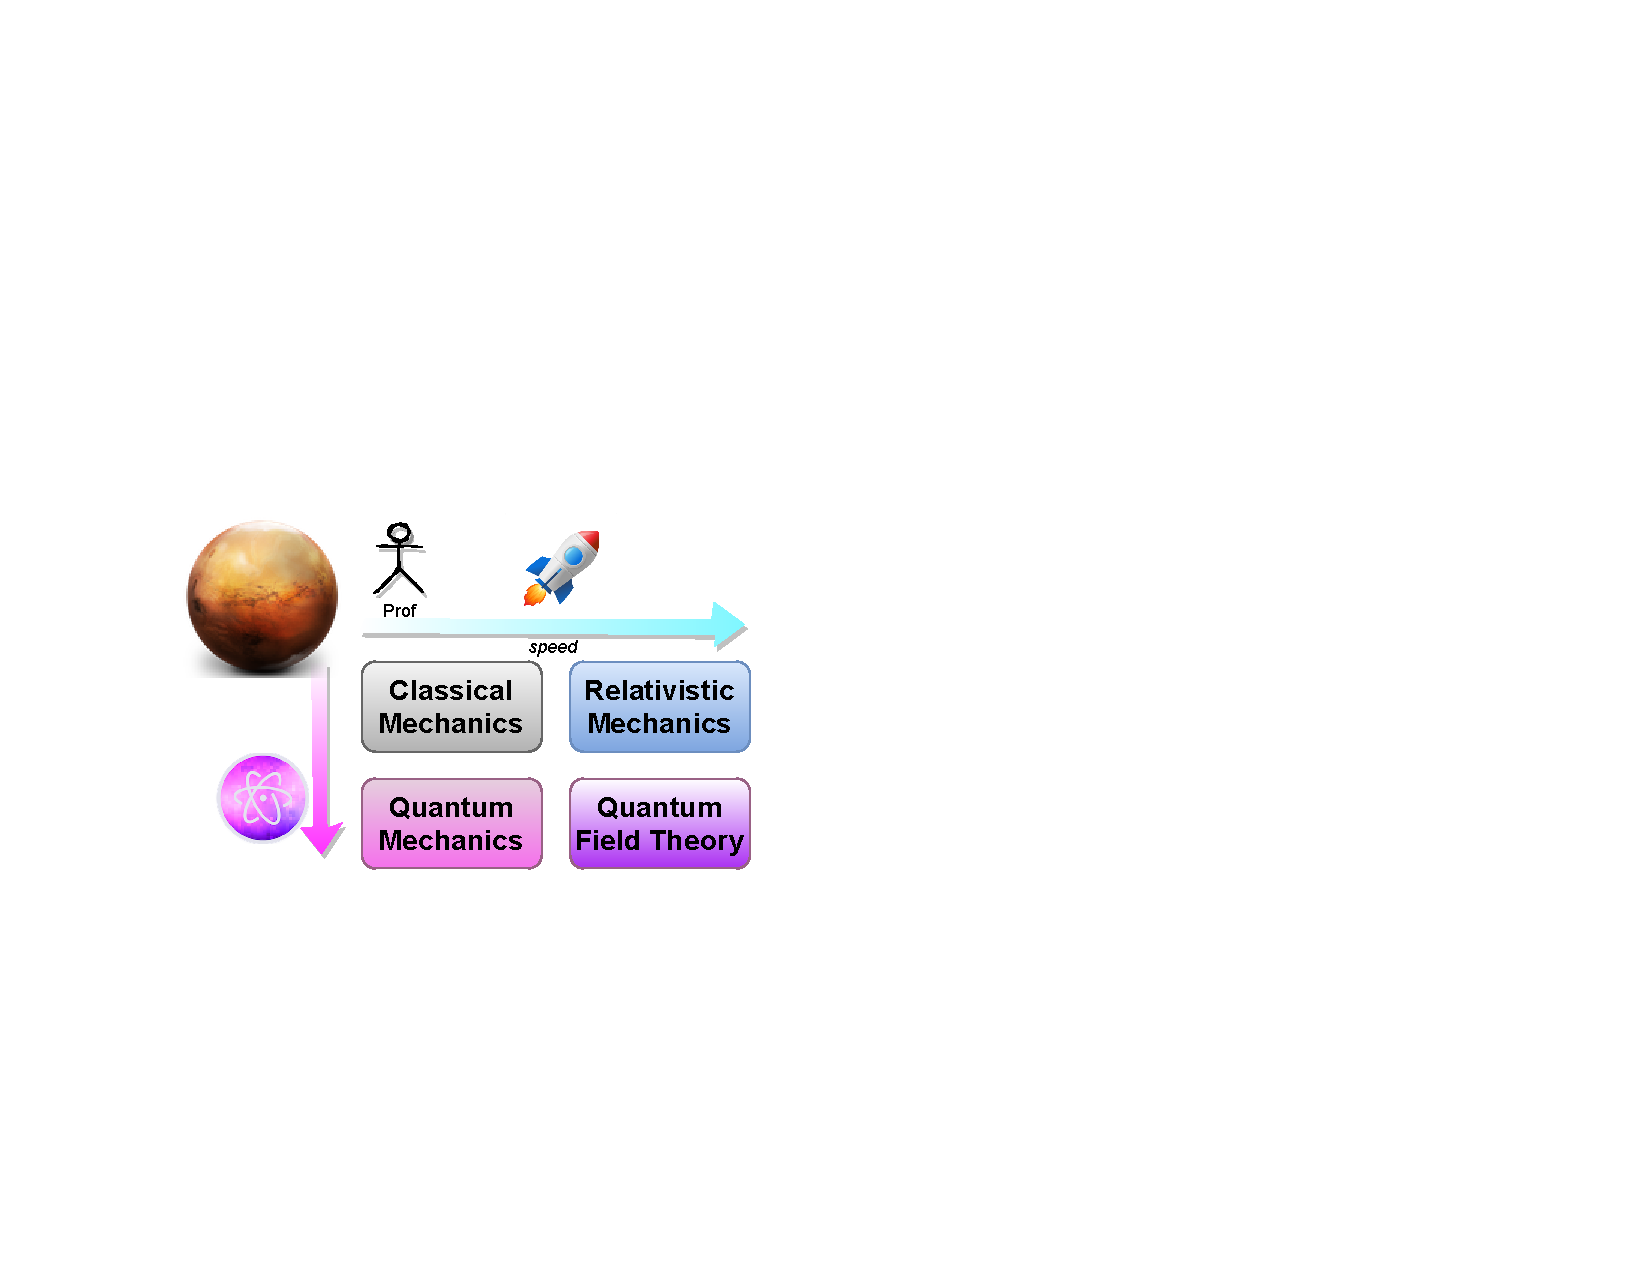
\includegraphics[width=\columnwidth]{stat-mech-overview.pdf}
\caption{EM waves in a black box with sides of length $L$}
\end{figure}


\begin{enumerate}
\item Basics of probability
\item mean, median, var, std, ...
\end{enumerate}


\clearpage
\section{Binary State Systems: April 2}

\clearpage
\section{Equilibrium: April 7}

\subsection{Review of Last Week}
\begin{itemize}
\item \textbf{Fundamental Assumption of Statistical Mechanics:} "An isolated system in uqilibrium is equally likely to be found in any of the microstates available to it."

\item $g =$ "the multiplicity"; the number of accessible micro states for a given set of extensive parameters (e.g. U, N, V)

\item If all such states are equally likely, then \textit{the probability distribution is uniform}: $P_i = 1/g$

\item The mean value or "Expectation value" of an observable $\mathcal{A}$ is defined 
  $\Braket{\mathcal{A}} = \displaystyle \sum_{i} \mathcal{A}_i P(i)$

\item Fluctuations are \textit{\textbf{tiny}}: For N >> 1, quantities like $\Delta U/U$ go as $1/\sqrt{N}$

\item This is a consequence of the Central Limit Theorem. Ensembles of many varying distributions sum up to a Gaussian distribution.

\end{itemize}

\subsubsection{Collection of N magnetic spins}
\begin{equation}
g(N,s) = \frac{N!}{(N/2 + s)! (N/2-s)!}
\end{equation}
Using Stirling's Approximation (cf. \href{http://mathworld.wolfram.com/StirlingsApproximation.html}{MathWorld}):
\begin{equation}
log(N!) = N log(N) - N + \frac{1}{2}log(2 \pi N)
\end{equation}
\begin{figure}[h]
\centering
\includegraphics[width=\columnwidth]{Figures/Stirling.pdf}
\caption{Comparison of various approximations to N!}
\end{figure}
after some substitutions, we find that

\begin{equation}
g(N,s) = 2^N \sqrt{\frac{2}{\pi N}} exp\bigg[-\frac{1}{2}\bigg(\frac{s}{\sigma_s}\bigg)^2\bigg]
\end{equation}
where $\sigma_s = \sqrt{N}/2$ is the standard deviation of the Gaussian probability 
distribution of $s$, the spin excess.

\subsection{Thermal Equilibrium for Two Systems}
Let us consider two non-interacting systems. Each system is a box with a collections of
spins. Box 1 has $N_1$ total atoms and an initial spin excess of $s_1$.
The combined multiplicity of these 
two systems (before we allow them to interact) is (using the same logic that we used to consider
our binary model of coin flips) just the product of the individual multiplicities:
\begin{align}
g_{tot} &= g_1 \times g_2 \\
        &= \frac{2}{\pi} \frac{1}{\sqrt{N_1 N_2}} 2^{N_1 + N_2} exp\bigg[-2\bigg(\frac{s_1^2}{N_1} + 
        \frac{s_2^2}{N_2}\bigg)\bigg]
\label{eq:ginit}
\end{align}
Rather than consider some artificial magnetic spin exchange interaction, let us instead
turn on an external magnetic field, such that the energy of each system becomes
$U_i = -2 m B s_i$, where $m$ is the magnetic moment of each atom and $B$ is the magnetic
field. We then bring the boxes into contact, such that it is possible to interchange energy
between the two system. The total spin and the total energy will remain conserved
(e.g. $U = U_1 + U_2$). For this two system example, we do not let the number of atoms in
each box change: $N_1 = const, N_2 = const$.

After the energy exchange begins, the two systems move from their 
initial state (Eq.~\ref{eq:ginit}) into a new state
\begin{equation}
g_{tot} = g_1(U_1^\prime) \times g_2(U_2^\prime)
\end{equation}
with more accessible microstates.

We would like to find what the new equilibrium state is. In other words, 
what is the most probable state after the two (sub)systems have been in contact 
long enough to come into equilibrium?
\begin{figure}[h]
\centering
\includegraphics[width=\columnwidth]{Figures/TwoSystemMultiplicity.pdf}
\caption{The multiplicity functions for two systems before (Blue and Red) and after (Purple) being put 
	into thermal contact.}
\end{figure}

To find this, we would like to find the stationary point for the combined multiplicity function. To do this we set the $dg/dU = 0$:

\begin{equation}
dg = \bigg(\frac{\partial g_1}{\partial U_1}\bigg)_{N_1} g_2~dU_1 +
     \bigg(\frac{\partial g_2}{\partial U_2}\bigg)_{N_2} g_1~dU_2 = 0  
\label{eq:maxg}
\end{equation}

Since energy is conserved, any energy gained by one sub-system is equal
to the amount lost by the other: $dU_1 = -dU_2$. Dividing through by
$g_1 g_2$, we find the condition for \textit{thermal equilibrium}:

\begin{equation}
\bigg(\frac{\partial log(g_1)}{\partial U_1}\bigg)_{N_1} = 
\bigg(\frac{\partial log(g_2)}{\partial U_2}\bigg)_{N_2}
\label{eq:maxmicro}
\end{equation}



\clearpage
\section{Entropy: April 9}

\subsection{Entropy}
\label{s:Entropy}
The number of microstates is a huge number! Its much easier to work with the
logarithm of such large numbers. The logarithm is also convenient since adding
systems together requires just adding their logarithms, rather than multiplying
the number of microstates.

So we define \textit{\textbf{entropy}} as:
\begin{equation}
\sigma \equiv log(g)
\end{equation}
This is a dimensionless (unitless) quantity (its just the logarithm 
of a large number...). \\

As we saw in the previous lecture, the combined system moves from its initial configuration
(where system 1 and 2 have the energies $U_1$ and $U_2$, respectively) into the one which
is \emph{overwhelmingly} likely. Recall that our conclusion from the discussion of thermal
equilibrium is that for macroscopic systems (e.g. with $N \gtrsim 10^{15}$...actually the
transition from micro to macro is a fuzzy concept, but this is an OK estimate for now), the
chances of the energy being even 1\,ppm different from the most probable value are astronomically unlikely (really? Yes - see the Shakespeare, monkeys, and typewriters
problem in this week's problem set).

\begin{equation}
\bigg(\frac{\partial \sigma_1}{\partial U_1}\bigg)_{N_1} = 
\bigg(\frac{\partial \sigma_2}{\partial U_2}\bigg)_{N_2}
\label{eq:Teq}
\end{equation}

This tendency of the system to always move into a configuration which maximizes
the number of accessible micro-states ($g$) is a just another way of stating the
2$^{\rm nd}$ Law of Thermodynamics: The entropy of a closed system will always 
increase until the system reaches equilibrium.

\epigraph{Turning and turning in the widening gyre \\
The falcon cannot hear the falconer; \\
Things fall apart; the centre cannot hold; \\
Mere anarchy is loosed upon the world,...}{\textit{William B. Yeats, 1919}}

\subsection{Temperature}
\label{s:Temperature}

Intuitively, we know that putting things in contact brings them to the same temperature
(cf. the "Brain Freeze" available at the Red Door Cafe). So we want this to be
implied by Eq.~\ref{eq:Teq}.

From Eq.~\ref{eq:Teq}, we could pick $\tau, 1/\tau, or -\tau,...$, but we want temperature
to correspond to our human definitions of it. Zero temperature should be very low energy
and temperature should rise as we put more kinetic energy into the particles, so we define
it like so:
\begin{equation}
\frac{1}{\tau} \equiv \bigg(\frac{\partial \sigma}{\partial U}\bigg)_{N}
\label{eq:Temp}
\end{equation}

\subsection{The Laws of Thermodynamics}

\subsubsection{The 0$^{\rm th}$ Law: Thermometers}
\href{http://en.wikipedia.org/wiki/Zeroth_law_of_thermodynamics}{Wikipedia:Zeroth Law}

From our definitions of temperature and thermal equilibrium 
(cf. \cref{eq:Temp,eq:Teq}), 
we see that if $\tau_1 = \tau_3$ and $\tau_2 = \tau_3$, then 
$\tau_1 = \tau_2$. 
In this example, $\tau_3$ is the temperature of the thermometer we are 
using to establish the equivalence of the temperatures of our two example 
systems (1 and 2). Why is this seemingly trivial statement worthy
of being a so-called "Law of Thermodynamics"? 



\subsubsection{The 1$^{\rm st}$ Law: No Free Lunch}
\begin{figure}[h]
\centering
\includegraphics[width=0.5\columnwidth]{Figures/Carnot_heat_engine_2.pdf}
\caption{Schematic diagram of Carnot's Heat Engine \\
	\url{http://commons.wikimedia.org/wiki/File:Carnot_heat_engine_2.svg}}
\end{figure}
A concise statement of the 1$^{\rm st}$ Law is:
\begin{equation}
\Delta U = Q + W
\label{eq:FirstLaw}
\end{equation}
where $\Delta U$ is the total internal energy of our system, $W$ is the
mechanical work done \emph{to the system}\footnote{note the sign convention
here; the work is done to the system and not by the system}, and $Q$ is
the \textit{heat}. But what is heat? We all know what it is intuitively,
but it is important to define it such that it can be used consistently in
our studies of statistical mechanics. As defined in Ch.~8 of the textbook,
heat is the energy transfer between two systems which are in thermal contact.
It does not include work or any transfer of material. In the Carnot example
above, $W = Q_H - Q_C$. Systems where $W > Q_H - Q_C$ are called
perpetual motion machines of the first kind, and are known to be
impossible to conservation of energy.

\subsubsection{The 2$^{\rm nd}$ Law: Everything Runs Down}
As we saw above in Sec.~\ref{s:Entropy}, when a system begins in a
non-equilibrium state (such as the one where we first bring the two
sub-systems into contact), it always moves in the direction which
increases the entropy:\footnote{This is put to music in the song "Unsustainable", from the rock band Muse's album "The 2nd Law". Some Gaussian distributions and combinatorics are displayed for affect in their music video:
\href{https://www.youtube.com/watch?v=EF_xdvn52As}{YouTube:Unsustainable}} pieces of a broken wine glass "never" reassemble
into a whole glass. When we run the film backwards, we see this happen,
but it seems that there is a preferred to direction to the 
flow of time. This is often referred to as the 
Arrow of TIme~\footnote{\href{http://www.wired.com/2014/04/quantum-theory-flow-time/}{2004 Wired article} on how quantum correlations may be the underlying basis for the arrow of time}

For the heat engine example above, $\Delta \sigma = Q_C/\tau_C - Q_H/\tau_H$.
In order for $\Delta \sigma$ to be positive, we must have $\tau_H > \tau_C$,
since $Q_H \ge Q_C$.



\epigraph{The law that entropy always increases, holds, I think, the supreme position among the laws of Nature. If someone points out to you that your pet theory of the universe is in disagreement with Maxwell's equations --- then so much the worse for Maxwell's equations. If it is found to be contradicted by observation --- well, these experimentalists do bungle things sometimes. But if your theory is found to be against the second law of thermodynamics I can give you no hope; there is nothing for it but to collapse in deepest humiliation.}
{\textit{Sir Arthur S. Eddington, 1928}}

\subsubsection{The 3$^{\rm rd}$ Law: Nernst Theorem}





\clearpage
\section{Boltzmann Factor: April 14}


\subsection{The Boltzmann Factor}
An important problem in Statistical Physics, is to find the probability
of finding a system in a state $s$ of energy $\epsilon_s$. We already
know how to do this for closed systems, but most systems are, in reality, open systems -- that is, they are in contact with a large thermal bath or reservoir. This might be the rest of the room (in the case of a tiny experiment) or the rest of the city (in the case that the system is a building) or even the rest of the universe (in astrophysical or cosmological cases). \\

So lets take our little system $\mathcal{S}$ and put in contact with our large reservoir $\mathcal{R}$ with initial energy $U_0$ and temperature $\tau_R$. Now we put our system in thermal (and later, mechanical) contact with the reservoir such that the new energy of the reservoir is $U_0 - \epsilon_s$. Now 
$\mathcal{R}$ can be in any of its $g_R(U_0 - \epsilon_s)$ microstates, just as we saw in last week's \textit{microcanonical} picture. \\

For a given state $s$, there is no degeneracy; the multiplicity, $g_s = 1$. So the probability of finding the total system ($\mathcal{S} + \mathcal{R}$) in the state where $\mathcal{S}$ has energy $\epsilon_s$, is just dependent on the multiplicity $g_R$: $P(s) \propto g_R(U_0 - \epsilon_s)$. Since 
$U_0 \gg \epsilon_s$, we can use the Taylor expansion to find a simplified form:

\begin{equation}
\log g_R = \sigma_R(U_0 - \epsilon_s) \simeq 
	\sigma_R(U_0) - 
	\epsilon_s \bigg(\frac{\partial \sigma_R}{\partial U_R}\bigg) +
	\mathcal{O}(\epsilon_s^2)
\end{equation}

Since $(\partial \sigma_R/\partial U_R) = 1/\tau_R$, we can rewrite the proportionality for the probability as:

\begin{equation}
P(s) \propto exp(-\epsilon_s/\tau_R)
\end{equation}

This is \textbf{one the most practically useful results in statistical physics}: it allows us to compute the relative probability of the system being in different energy states. This expression, $exp(-\epsilon_s/\tau_R)$, is called the
\emph{Boltzmann Factor}.


\subsection{Partition Function}
We would like to normalize the probability so that 
$\sum_s P(s) = 1$. To do this, we just sum over all possible energy states.

\begin{equation}
P(s) = \frac{exp(-\epsilon_s/\tau_R)}{\sum_s exp(-\epsilon_s/\tau_R} = 1
\end{equation}
and where we will define the \emph{Partition Function}\footnote{an oddly named function for sure} as
\begin{equation}
Z(\tau_R) \equiv \sum_s exp(-\epsilon_s/\tau_R
\end{equation}

\subsection{Pressure}

\subsection{Free Energy}


\textbf{Summary}

\begin{itemize}
\item The probability of finding a system (in microstate $s$ with
	energy $\epsilon_s$, in thermal equilibrium with a reservoir 
	at temperature $\tau_R$) is proportional to the 
	\emph{Boltzmann factor} $P(s) \propto exp(-\epsilon_s/\tau_R)$.

\item To normalize $P(s)$ properly ($\sum_{s} P(s) = 1$), we divide
	the Boltzmann factor by the sum over all energy states.
	$P(s) = exp(-\epsilon_s/\tau_R)/Z$, where 
	$Z(\tau_R) \equiv \sum_{s} exp(-\epsilon_s/\tau_R)$. $Z$ is called the
	partition function.

\item For a compressible system, if we change the volume slowly and by
	a small amount, the entropy won't change (\textit{isentropic}). This
	is defined as \textit{pressure}: $p = -(\partial U/\partial V)_\sigma$

\item The picture of closed system with an accessible number of microstates
	and associated entropy is the \emph{microcanonical ensemble}. In this picture, the energy, volume, and number of the system is fixed.

\item The \emph{canonical ensemble} is the similar picture, but with 
	the system now in thermal equilibrium with a heat bath. Consequently,
	the temperature is now fixed, but the energy of the system is not.

\end{itemize}






\clearpage
\section{Helmholtz Free Energy and the Ideal Gas: April 16}

\clearpage
\section{Ideal Gas I: April 16}
\label{s:IdealGasI}
As a first look at the Ideal Gas model, we start by assuming that we have $N$ identical point like particles in a box. These particles do not interact with each other and, by the virtue of being point-like, we can ignore the rotational and vibrational energies which real molecules have.\\

We can then procede to solve for the quantum wavefunctions and energies just as we do for the standard "particle-in-a-box" problem (cf. K\&K, Ch.\,1, pp.\,9-10).
\begin{equation}
\hat{H} \Braket{\Psi} = E \Braket{\Psi}
\end{equation}

\begin{figure}[h]
\centering
\includegraphics[width=0.7\columnwidth]{Figures/ParticleBoxPlot.pdf}
\caption{Example wavefunction for a particle in a square 2D box 
	with sides of length $L$}
\end{figure}

For this potential (the box), the Hamiltonian is just that for a free 
particle:

\begin{equation}
\hat{H} = -\frac{\hbar^2}{2 m} \nabla^2
\end{equation}

This type of wave equation has solutions of the form $A \sin{x} + B \cos{x}$.
By including the boundary conditions that $\Braket{\Psi} = 0$ when
($x, y, z$) = $0$ or $L$, we can eliminate the cosine terms and we are left
with:
\begin{equation}
\Psi(x,y,z) = \mathcal{C} \sin(n_x \frac{\pi}{L} x) \sin(n_y \frac{\pi}{L} y) \sin(n_z \frac{\pi}{L} z)
\end{equation}
where $\mathcal{C}$ is the normalization constant. After normalization (to set the total probability equal to 1), we can get the quantized energies by plugging into the Schr\"odinger Equation above:
\begin{equation}
\epsilon_n = \frac{\hbar^2}{2 m}\bigg(\frac{\pi}{L} \bigg)^2 (n_x^2 + n_y^2 + n_z^2)
\label{eq:IdealGasEnergies}
\end{equation}

\subsection{Partition Function}
We can now begin using our standard canonical ensemble 'toolbox' to derive relationships for the macroscopic observables of the system. The Boltzmann factor for a single particle is just $exp(-\epsilon_n/\tau)$ and the Partition function is
\begin{equation}
Z_1 = \sum_{n_x} \sum_{n_y} \sum_{n_z} e^{-\epsilon_n/\tau}
\end{equation}
Unsurprisingly, we would like to convert this summation into an integral in order to solve it, but is this really valid? It is, but only if the error between the sum and the series is small; i.e. true if $\epsilon_{n+1} - \epsilon_n \ll \tau$. 
At room temperature, $\tau = k_B T = (1.38 \times 10^{-23} J/K)(300 K)$. 
To convert to eV, we divide by the electron charge ($1.602 \times 10^{-19} C$), 
so $\tau \simeq \frac{1}{40} eV$. The
prefactor in \cref{eq:IdealGasEnergies} is $\sim 10^{-16} eV$ for a $1~mm^3$ box,
so the approximation made by using an integral instead of an infinite series is extremely accurate even at the nano-Kelvin temperature now achievable through modern cryogenic methods.\\

We can then perform the integral by noting that its separable into three integrals (one for each $n_i$) and that each integral is of the form $\int exp(-\alpha^2 x^2)$, which we have done before and can look up in Appendix A of K\&K or 
\href{http://www.wolframalpha.com/input/?i=integrate\%20exp(-a\%5E2\%20x\%5E2)\%20from\%20x\%3D0..infinity}{Wolfram Alpha}.
\begin{align}
Z_1 &= L^3 \bigg(\frac{2 \pi \hbar^2}{m \tau}\bigg)^{-3/2} \\
    &= n_Q V
\end{align}
where $V = L^3$ and 
\begin{equation}
n_Q \equiv \bigg(\frac{2 \pi \hbar^2}{m \tau}\bigg)^{-3/2}
\label{eq:QuantConc}
\end{equation} 
which we define as the \emph{Quantum Concentration}. Since 
for most gases at
room temperature, the single particle density ($1/V$) is much smaller than
$n_Q$, $Z_1 \ll 1$, and the \textit{classical approximation} is valid. Otherwise, we would have to consider the quantum entanglement between the molecules.\\

For distinguishable particles, the multi-particle partition function is just the product of the individual particle partition functions, just as the multi particle multiplicity is the product of the single particle multiplicities. Since the
gas particles are identical, we weight it by the number of identical permutations:
\begin{equation}
Z_N = \frac{Z_1}{N!} = \frac{(n_Q V)^N}{N!}
\label{eq:IdealGasZ}
\end{equation}



\subsection{The Ideal Gas Law}
To understand the macroscopic properties of the N particle ideal gas, we can start with our expression for the Free Energy in terms of the Partition Function:
\begin{align}
F &= -\tau~\log Z_N \\
  &= -\tau~(N \log Z_1 - \log N!) \\
  &= -\tau~(N \log{n_Q V} - \log N!)
\end{align}

From \cref{eq:dFdX}, we have that
\begin{align}
p &= -\bigg(\frac{\partial F}{\partial V}\bigg)_\tau \\
  &= N \tau / V
\end{align}
and changing from our 'fundamental' units to SI units, we recover the Ideal Gas Law:
\begin{equation}
\boxed{p V = N k_B T}
\end{equation}





















\clearpage
\section{Planck Black Body: April 21}

Let's consider now a system which is similar to the previous two (Ideal Gas and small System in a large Reservoir), but with a significant twist. Instead of a system where the constituents have a mass, we want to study what happens inside of a 
black\,\footnote{Here, by 'black', I mean that the walls of the box are a 'perfectly' absorbing conductor. This is a little counterintuitive; you know that very good conductors (e.g. aluminum, copper, silver) are very reflective and \emph{not} perfectly absorbing. Nevertheless, this turns out to be a valid approximation for what we are looking into and, in fact, works well with boxes of almost any generic properties.} box in thermal equilibrium with a Reservoir. Instead of particles of a gas, we will be working with \textit{photons}, the massless quanta of electromagnetic radiation. In the end we would like to end up with all the now usual concepts: total energy, entropy, pressure (yes, even light has a 
pressure~\footnote{cf. solar sails}), and the energy distribution (i.e. can 
we predict what color something will be?). \\

\begin{figure}[h]
\centering
\includegraphics[width=0.3\columnwidth]{Figures/245px-photon_waves.png}
\caption{EM waves in a black box with sides of length $L$}
\end{figure}


We'll start off with the assumption\,\footnote{which will be qualified later} that the energy of each photon of angular frequency $\omega$($=2 \pi \nu$) will just be proportional to the frequency:
\begin{equation}
\epsilon = \hbar \omega
\end{equation}
To an extremely good approximation, photons do not interact with each other (i.e. you cannot deflect a laser beam with another laser beam). So there can, in principle, be many photons with the same energy inside the box. We'll denote the occupancy of each mode as $s$, and so the energy per mode will be $\epsilon_s = s \hbar \omega$. The total energy will then just be an appropriately weighted sum over all the available modes.\\

At a temperature $\tau$, the Boltzmann factor for a \textit{single} mode 
is $e^{-s \hbar \omega / \tau}$. So the partition function for that mode is:
\begin{align}
Z &= \sum_{s=0}^{\infty} e^{-s \hbar \omega / \tau} \\
  &= \frac{1}{1 - e^{-\hbar \omega / \tau}}
\label{eq:PartPlanck}
\end{align}
where we have used the relation $\sum_{s=0}^{\infty} x^s = 1/(1-x)$, 
valid when $x < 1$. \\

\subsection{The Planck Distribution}
At this point we can utilize all of the tools we have developed during the study of the canonical ensemble in Chapter 3. We know that the probability 
distribution can just be computed from the Boltzmann factor and the partition 
function (cf.\,\cref{eq:PofS}):
\begin{equation}
P(s) = e^{-s \hbar \omega / \tau} \bigg[ 1 - e^{-\hbar \omega / \tau} \bigg]
\end{equation}
and to find the average occupancy of each mode we just multiply by $s$ and sum over all states:
\begin{align}
\Braket{s} &= \sum_{s=0}^{\infty} s~P(s) \\
           &= \frac{1}{Z} \sum_{s=0}^{\infty} s~e^{-s \hbar \omega / \tau}
\end{align}
We can perform the sum here by transforming it into a more familiar form. To do this note that:
\begin{equation}
\sum s~e^{-s x} = -\frac{d}{dx} \sum e^{-s x}
\end{equation}
and the right hand side can be summed in the same way as \cref{eq:PartPlanck}, above.
So finally we arrive at the expression for the average occupancy:
\begin{equation}
\boxed{\Braket{s} = \frac{1}{e^{\hbar \omega / \tau} - 1}}
\end{equation}
which is the \emph{Planck distribution} for the occupancy of a single mode in thermal equilibrium with a heat bath of temperature $\tau$. The average energy in each mode is:
\begin{equation}
\boxed{\Braket{\epsilon} = \Braket{s} \hbar \omega= 
\frac{\hbar \omega}{e^{\hbar \omega / \tau} - 1}}
\end{equation}
Its interesting to look at the high and low temperature (or equivalently, the low and high frequency) limits of this expression. \\

At high temperatures, where 
$\tau \gg \hbar \omega$, we can expand the denominator ($e^x \simeq 1 + x$) and see
that $\Braket{\epsilon} \to \tau$. This is the 'classical limit'; the energy is just
proportional to the temperature and there is no evidence of quantization.\\

At low temperatures, where $\tau \ll \hbar \omega$, the denominator becomes large
and $\Braket{\epsilon} \to 0$. So a black box will tend towards zero energy in the
electromangetic field~\footnote{neglecting the ground state energy of 
$\frac{1}{2}\hbar \omega$ per mode} as well as zero occupancy. \\

This highlights another interesting difference between
a box of ideal gas molecules and a box of radiation: \emph{the photon number is
not a conserved quantity}. As we will see soon, the same is true for 
\textit{phonons}, the acoustic excitations in a solid.


\subsection{The Stefan-Boltzmann Law}
We would like to now move on to the main goal, which is to find the total energy,
entropy, etc. for the blackbody, summing over all the modes.

\begin{equation}
U = 2 \sum_n \Braket{\epsilon_n} = 
\sum_n \frac{\hbar \omega_n}{exp(\hbar \omega_n / \tau) - 1}
\end{equation}
where we have followed the convention from K \& K pp. 92-93 which describes
the accounting for the modes allowed in the box (similar reasoning as we use
for waves on a string and particle in a box). The factor of 2 comes from accounting
for the 2 polarizations of the radiation field and $\omega_n = n \pi c/L$.\\

We can replace the sum over the indices ($n_x, n_y, n_z$) with a triple integral
to make the computation easier. This is valid as long as the box is not small
with respect to the wavelength of the relavent radiation field ($L \gg c/\omega$).\\

To make the integral easier, we'll convert it from Cartesian coordinates to
spherical coordinates and replace the volume element $dn_x dn_y dn_z$, with
the spherical volume element $4 \pi\,n^2 dn$.
\begin{align}
U &= 2 \times \frac{1}{8} \times 4 \pi 
\int_{0}^{\infty} n^2 \frac{\hbar \omega_n}{exp(\hbar \omega_n / \tau) - 1} dn \\
  &= \frac{L^3 \tau^4}{\pi^2 \hbar^3 c^3} \int_{0}^{\infty} \frac{x^3}{e^x - 1} dx \\
  &= \frac{\pi^2 L^3 \tau^4}{15 \hbar^3 c^3}
\label{eq:BBenergy}
\end{align}
where the factor of 2 is for both polarizations, the $1/8$ because we only want to consider one octant of the spherical volume (where the wavenumbers are positive), and the $4 \pi$ covers the angular part of the volume integral. We then have made the substitution $x = \pi \hbar c n / L \tau$ to get the dimensionless 
integral. We can look up~\footnote{you can do it for yourself in a few steps if you want: multiply top and bottom by $e^{-x}$ and then recall our infinite sum for 
$1/(1-x)$} the integral in a book or Mathematica to find that its $\pi^4/15$.

Its useful to also look at the spectral distribution of the energy. To get that
we can rewrite the integrand above as:
\begin{align}
\frac{U}{V} &= \int_{0}^{\infty} u_{\omega} d\omega \\
	        &= \frac{\hbar}{\pi^2 c^3} \frac{\omega^3}{e^{\hbar \omega/\tau} - 1}
\end{align}
where we've moved the volume ($V = L^3$) over to the left hand side and used
our expression from above to replace $n$ with $\omega$. This
\textit{spectral density}, $u_{\omega}$, is called the
\emph{Planck Black Body Spectrum} and the theoretical and experimental work which
gave rise to it was the first evidence for $\hbar$ and was the birth of
Quantum Mechanics.

\begin{figure}[ht]
\centering
\includegraphics[width=0.7\columnwidth]{Figures/BlackbodySpectrum_loglog_150dpi_en.png}
\caption{Blackbody Radiation Intensity Spectral density. \\
	From \url{https://commons.wikimedia.org/wiki/File:BlackbodySpectrum_loglog_150dpi_en.png}}
\end{figure}



%\clearpage
%\section{Ideal Gas: April 16}
Introduction to the Ideal Gas model.

\clearpage
\section{Chemical Potential: April 28}
We have so far studied systems in which the volume and temperature are allowed to vary. In the microcanonical ensemble of chapters 1 \& 2, we used the Fundamental Postulate of Statistical Mechanics:\\
\\
\doublebox{An isolated system in equilibrium is equally likely to be found in any of its available microstates.}\\
\\
to find the most probable state. In the canonical ensemble we were introduced to the concepts of the Helmholtz Free Energy, the Boltzmann Factor, and the Partition Function. This was useful in describing the behavior of a system in thermal equilibrium with another system (often a very large Reservoir or Heat Bath).\\

We could also imagine allowing the volume or the number of particles to change. We have already seen an example of this in the blackbody radiation case -- there the number of particles was \textit{not conserved}.\\

Here we would like to consider the case where the particle number \emph{is} conserved, but where we allow the particles (as well as the thermal energy)to flow between the two systems, $\mathcal{S}_1$ and $\mathcal{S}_2$. 
This is called \textit{diffusive contact}. 
We will use the tools developed for the canonical ensemble here again.
Some examples where this will be a useful picture:
\begin{itemize}
\item Permeable membrane between two boxes of gas.
\item Adsorption / contamination of a gas onto a surface, such as might occur in thin film deposition or contamination of a silicon wafer in a clean room environment.
\item Flow of particles in a gravitational field: barometric pressure or relative gas concentration in the Earth's atmosphere.
\item ...
\end{itemize}


Just as before, when we only had thermal contact, the 
free energy ($F = -\tau \log{Z}$) will be minimized when the two
systems come to equilibrium; i.e. when the two non-equilibrium
systems are allowed to diffuse into each other, they will change
particle concentrations in the way that \textit{minimizes the total
free energy}: $F = F_1 + F_2$. To find the minimum, we set the differential equal to zero:
\begin{align}
dF &= \bigg(\frac{\partial F_1}{\partial N_1}\bigg) dN_1
	- \bigg(\frac{\partial F_2}{\partial N_2}\bigg) dN_1 \\
   &= (\mu_1 - \mu_2) dN_1 = 0
\label{eq:ChemEquil}
\end{align}
where we have used the total particle number conservation ($N = N_1 + N_2$)
to set $dN_1 = -dN_2$. We can define the \textit{chemical potential}:
\begin{equation}
\boxed{\mu \equiv \bigg(\frac{\partial F}{\partial N}\bigg)_{\tau,V}}
\label{eq:ChemPot}
\end{equation}

If we start off near equilibrium, and a small amount of particles, 
$dN_1 > 0$, is moved from $\mathcal{S}_2$ to $\mathcal{S}_1$ to
bring the system closer to equilibrium, we know that $F$ should get smaller:
\begin{align}
dF &= d(F_1 + F_2) < 0 \\
   &= (\mu_1 - \mu_2) dN_1 < 0
\end{align}
so it must be that $\mu_1 < \mu_2$. The particle flow is from a region of
higher to lower chemical potential. As long as we're treating the system as if the particles are non-interacting, we can also assert that the particles of one species do not effect the others and so a system with a collection of different kinds of particles will have a chemical potential for each kind:
\begin{equation}
\mu_i = \bigg(\frac{\partial F}{\partial N_i}\bigg)_{\tau,V,N_{i \neq j}}
\end{equation}


\subsection{Ideal Gas}
From \cref{s:IdealGasI}, we have the expression for the Ideal Gas
Partition function (cf.~\cref{eq:IdealGasZ}) and the Quantum 
Concentration (cf.~\cref{eq:QuantConc}). Using Stirling's 
approximation (cf.~\cref{eq:Stirling}) we can write the Free Energy
as:
\begin{align}
F &= -\tau \log{\frac{Z_{1}^N}{N!}} \\
  &= -\tau \bigg[N \log{n_Q V} - N \log{N} + N \bigg] 
\end{align}
and the chemical potential is then:
\begin{align}
\mu &= \bigg(\frac{\partial F}{\partial N}\bigg)_{\tau,V} \\
    &= -\tau~(\log{n_Q V} - \log{N}) \\
    &= \tau \log{\frac{n}{n_Q}}
\end{align} 
where $n \equiv N/V$ is the number density for the gas 
particles (molecules). Since, for the ideal gas, $n \ll n_q$, the
chemical potential will always be very negative. An ideal gas
with a higher number density will have a more positive potential
and so the particles will flow from the system of high density
into the system with low density, just as your intuition would
tell you.


\subsection{Barometric Pressure in the Earth's Atmosphere}
As an example of the utility of the chemical potential, we can examine
a simplified model of the atmosphere. Assume that the atmosphere
is in thermal and chemical equilibrium. To simplify the problem,
will assume that there is no significant temperature gradient for the
regions that we are considering (in reality, of course, higher
altitudes are much colder and there is often wind and turbulence).

In addition to the internal chemical potential, $\mu_{int}$, there is
an external potential,$\mu_{grav} = m g h$, due to gravity. If the lower
and upper atmosphere are in equilibrium, we must set these to be equal.
\begin{align}
\mu_{total} = \tau \log{n(h)/n_Q} = \tau \log{n(0)/n_Q}
\end{align}
Solving for $n(h)$, we find:
\begin{align}
n(h) &= n(0) e^{-m g h / \tau} \\
p(h) &= p(0) e^{-m g h / \tau}
\end{align}
since, for an ideal gas, $p = n \tau$.

\clearpage
\section{The Grand Canonical Ensemble: April 30}

\textbf{Microcanonical Ensemble:} An isolated system. No thermal, mechanical, or diffusive contact with the outside world. For example, when we considered applying a magnetic field to the isolated system of spins, we did not take into account the effect this had on the thing producing the field.\\

\textbf{Canonical Ensemble:} The system is connected to a heat bath. The temperature of the heat bath is not effected by the connection - its assumed that the heat bath (reservoir) is large in comparison with the system so that its temperature is not changed by contact.\\

\textbf{Grand Canonical Ensemble:} In this model, we allow both thermal and diffusive contact. The reservoir determines the temperature of the combined system and the total number of particles is fixed, but the particles are allowed to flow between system and reservoir.\\

Given the added property of diffusion, we can now bring into action the techniques we used to arrive at the canonical ensemble picture. So we'd like to come up with formulae analagous to the Boltzmann 
factor (\cref{s:BoltzmannFactor}) and the 
Partition Function (\cref{s:PartitionFunction}).\\

\subsection{The Gibbs Factor}
For a given microstate $\mathcal{S}$ of our system, it will have $N$ particles and an energy $\epsilon_S$. The probability that our system is in this particular microstate is:
\begin{equation}
P(N,\epsilon_S) \propto
g_{\mathcal{R}}(U_0-\epsilon_S, N_0-N) g_{\mathcal{S}}(\epsilon_S,N)
\label{eq:Pgrand1}
\end{equation}
where $g_{\mathcal{S}}(\epsilon_S,N) = 1$ since this is for a precisely
defned microstate (i.e. not an ensemble of microstates corresponding to a particular macrostate).

Since $N \ll N_0$ and $\epsilon_S \ll U_0$, it is reasonable to simplify our expression by taking the Taylor expansion of the 
entropy ($\sigma_{\mathcal{R}} = \log{g_{\mathcal{R}}}$), just as we did for the Boltzmann factor.
\begin{align}
\sigma_{\mathcal{R}}(U_0-\epsilon_S, N_0-N) &\simeq 
\sigma_{\mathcal{R}}(U_0, N_0)
-\epsilon_S \bigg(\frac{\partial \sigma_{\mathcal{R}}}{\partial U}\bigg)_N
-N \bigg(\frac{\partial \sigma_{\mathcal{R}}}{\partial N}\bigg)_U
+ \mathcal{O}(U^2) + \mathcal{O}(N^2) +... \\
       &= \sigma_{\mathcal{R}}(U_0, N_0) - \frac{\epsilon_S}{\tau} + 
       \frac{\mu~N}{\tau}
\end{align}
where we have used our knowledge of partial derivatives of entropy to express the entropy in terms of the temperature and the chemical potential. So we can now rewrite \cref{eq:Pgrand1} as:
\begin{equation}
P(N,\epsilon_S) = 
\frac{e^{-\epsilon_{S}/\tau + \mu N/\tau}}{\mathscr{Z}}
\end{equation}
where the factor $e^{\sigma_{\mathcal{R}}(U_0, N_0)}$ has been absorbed into the normalization factor in the denominator. The exponential in the numerator
is called the \emph{Gibbs factor}. It is the analog of the Boltzmann factor for a system in which the particle number is not fixed.

\subsection{The Grand Partition Function}
Since we want the above equation to be normalized such that 
$\sum P(N,\epsilon_S) = 1$, the normalization factor must be
\begin{equation}
\mathscr{Z} = \sum_{N=0}^{\infty} \sum_{s(N)} e^{-\epsilon_{S}/\tau + \mu N/\tau}
\end{equation}
which is just the sum over all possible states and numbers of particles of the Gibbs factor. This normalization function is called the 
\emph{Grand Partition Function} or sometimes the Gibbs sum.


\subsection{Maxwell Relations}
\label{s:MaxwellRelations}





\subsection{Fugacity}
\label{s:Fugacity}
\begin{figure}[h]
\centering
\includegraphics[width=8cm]{Figures/fugacity04.jpg}
\caption{\url{http://www.nzepc.auckland.ac.nz/features/fugacity/}}
\end{figure}



\begin{figure}[h]
\centering
\includegraphics[width=\columnwidth]{Figures/fugacity_ngrams.png}
\caption{The popularity of the word 'fugacity' over the years. Plot made using Google NGram Viewer. \url{http://www.informationisbeautiful.net/visualizations/google-ngram-experiments/}}
\end{figure}

\clearpage
\section{Ideal Quantum Gases: May 5}
A few weeks ago (cf. \cref{s:IdealGasI}), we did a first pass at examining the 
Ideal Gas:
\begin{itemize}
\item N identical particles in a box.
\item the particles are do not interact with each other
\item the particles are point-like; no rotational or vibrational modes
\end{itemize}

We then used the expression for the quantized energy levels based on the
'particle-in-a-box' Hamiltonian and found the Partition function (in the 
Canonical Ensemble representation) and expressions for the Quantum
Concentration and the Free Energy of the Ideal Gas. Now we want to look
at this in more detail, taking into account quantum mechanics and showing
how we recover the classical ideal gas behavior in the limit of high temperatures or low concentration.\\

In K\&K, the term 'orbital' denotes a particular state. It is motivated by
the meaning of orbital in the case of an atom, where each set of quantum
numbers refers to a unique quantum state. For the more general use in
statistical physics, we'll use the term 'orbital' even when there are
particles with no nucleus to orbit.\\

We use $n_i$ to refer to the occupancy of the $i^{th}$ state with 
energy $\epsilon_i$. The total quantum state of our system is fully specified by knowledge of $n_i$. With that information we can proceed to employ all of the
statistical mechanics tools that we have developed over the term to calculate
expressions for the behavior.\\

Our only constraints are that $\sum_i n_i = N$ (the total number of particles is fixed) and that the total energy of each microstate is given by:
\begin{equation}
\epsilon_s = \sum_i n_i \epsilon_i
\end{equation}

We will examine the case for three different kinds of particles:
\begin{enumerate}
\item Distinguishable particles, i.e. "classical" particles
\item Fermions: $n_i = 0$ or $1$
\item Bosons: $n_i = 0,1,2,3,...$
\end{enumerate}
these yield, respectively, Maxwell-Boltzmann, Fermi-Dirac, and Bose-Einstein
statistics.

\subsection{Ideal Gas}
With $N$ particles in a box, we consider a single orbital to be our system and the rest of the orbitals to be the reservoir. Since particles can move between orbitals, we will consider the system to be in \emph{diffusive and thermal} contact with the reservoir. This is where the use of the Grand Canonical ensemble comes into play. The Grand Canonical partition function is given by the sum over all possible states and numbers of particles of the Gibbs factor:
\begin{align}
\mathscr{Z} &= \sum_{N=0}^{\infty} \sum_{s(N)} e^{-\epsilon_{S}/\tau 
	+ \mu N/\tau}\\
            &= \sum_N \lambda^N \sum_s e^{-\epsilon_{S}/\tau}
\end{align}

In the case of $N$ indistinguishable particles, we found that the sum over the states (which is just the $N$ particle Partition function) is $Z_1^N/N!$. So for the ideal gas we can see that the Grand Canonical partition function is:
\begin{align}
\mathscr{Z} &= \sum_N \lambda^N \frac{Z_1^N}{N!} \\
	        &= e^{\lambda Z_1}
\end{align}
using the expression $e^x = \sum x^N/N!$ to simplify the equation. As before, we can find the thermal average number of particles by 'integrating' our observable, $N$, by the distribution. This gives us (after some algebra):
\begin{align}
\Braket{N} &= \tau \frac{\partial \log{\mathscr{Z}}}{\partial \mu}\\
	       &= \lambda Z_1
\end{align}
Using our expressions for the fugacity ($\lambda = n/n_Q$) and the single particle Partition function ($Z_1 = V n_Q$), we just recover the obvious result that $\Braket{N} = N$. Which is a reassuring confirmation that this approach is valid.

\subsection{Dilute Fermi Gas}








\clearpage
\section{Fermi Dirac Statistics}






\clearpage
\section{Bose Einstein Statistics: May 14, 19}






\clearpage
\section{Heat and Work: May 19}
\label{s:HeatWork}
This week, the objective is to study how heat and work behave in exchange between systems so that we can understand how practical devices work.\\

For a system with fixed number of particles $N$, the total internal energy can be expressed as a function of the entropy and volume:
\begin{equation}
dU = \tau d\sigma - p dV
\end{equation}
where the negative sign in the second term indicates that this is work done \textit{by} the system on the environment (it decreases the energy of the system). \emph{Decreasing} the volume of the system \emph{increases} its internal energy.

For a system with fixed $N$, there are a number of different ways to perform work on a system other than the obvious mechanical way of compression/expansion (such as changing the external magnetic field).

\subsection{Heat Engines}
\begin{figure}[h]
\centering
\includegraphics[width=0.7\columnwidth]{Figures/HeatEngineTable.png}
\caption{Comparison of Heat Engine Properties}
\end{figure}

There are illuminating Flash animations of a few different heat engines from Don Ion at Santa Barbara:
\url{http://science.sbcc.edu/~physics/flash/index.html}. The Carnot cycle is described in the textbook,
the 4-stroke engine (Otto) is the basic model of today's internal combustion engine in many cars, and
the Stirling cycle, which is very popular recenly due to its high efficiency and closed cycle operation.

\subsubsection{The Carnot Cycle}
The Carnot Cycle (named after Sadi Carnot) is an ideal version of a heat engine. A system (the engine) sits between a hot reservoir and a cold reservoir. Heat, $Q_h$, is extracted from hot reservoir at temperature $\tau_h$ and used to do some work. The system then ejects heat, $Q_l$, into a cold reservoir at temperature $\tau_l$ and then returns to its initial position. In the ideal Carnot picture, the engine is unchanged by this process and so the entropy remains constant: $\sigma_h = \sigma_l$

The amount of work done by the engine can, at best, be the difference in the heat extracted and the heat which is dumped to the cold reservoir.

\begin{equation}
W = Q_h - Q_l = \frac{\tau_h - \tau_l}{\tau_h} Q_h
\end{equation}

the \textit{Carnot efficiency} is defined as the ratio of the work done to the heat extracted from the reservoir:
\begin{equation}
\eta \equiv \frac{W}{Q_h} = 1 - \tau_l/\tau_h
\end{equation}

The P-V and T-S diagrams (from Thermopedia \url{http://dx.doi.org/10.1615/AtoZ.c.carnot_cycle})
\begin{figure}[h]
\centering
\includegraphics[width=0.7\columnwidth]{Figures/CarnotLoops.png}
\caption{Carnot cycle in P-V and T-S planes}
\end{figure}
give graphical representations of the amount of work done.

\begin{enumerate}
\item The system begins at low temperature and low entropy. The system 
	is compressed adiabatically (isentropically) and the temperature 
	increases to $\tau_h$.

\item At constant temperature $\tau_h$, heat $Q_h$ is injected into the 
	system (increasing its entropy) and the system expands along the 
	2 to 3 isotherm of the figure above.

\item The system is allowed to expand isentropically, going from $\tau_h$ to $\tau_l$

\item Heat, $Q_l$, is extracted from the system as it moves back 
	into its initial position.

\end{enumerate}


\subsection{Refrigeration}
Refrigeration is very nearly the opposite of the heat engine, when viewed in this diagramatic way. The equivalent efficiency is called the \emph{coefficient of refrigerator performance}:
\begin{equation}
\gamma_c = \frac{\tau_l}{\tau_h - \tau_l}
\end{equation}
which is not to be confused with our other symbol, $\gamma$, which is the adaibatic coefficient for an ideal gas.

\subsection{Path Dependence}
Using our knowledge of the ideal gas law, we can now compute the energy exchanges made during the isothermal and isentropic portions of the Carnot cycle.


\subsection{Otto Cycle (gasoline)}
The Otto cycle is interesting to us because it describes the behavior of the the 4-stroke internal combustion engine powering most of Los Angeles traffic.

\subsection{Stirling Engine}
The Stirling Engine is a closed cycle heat engine with the internal working fluid being manipulated through contact with a hot and cold surfaces. It is a very high efficiency engine which does not rely on combustion. It can use any heat source (such as renewables) and can be made to work very quietly. 


\subsection{Chemical Work}
What about when we transform particles from one type to another?


\subsection{Thermodynamic Impossibilities}
One of the practical uses of a knowledge of thermodynamics is the ability to debunk scientific frauds in the form of impossible heat engines, perpetual motion machines, devices which produce 'free energy' from the 'energy of empty space', etc.

\begin{itemize}
\item The Incredible Hulk: where does he get his mass from?

\item \url{http://io9.com/new-test-suggests-nasas-impossible-em-drive-will-work-1701188933}


\end{itemize}

\clearpage
\section{The Early Universe: May 26}
Now that we have covered several of the techniques for deriving thermodynamic observables from the fundamentals of statistical mechanics, we can apply these tools to describe some of the features of the early universe (post Big Bang).


\subsection{The Big Bang}
The actual Big Bang and the first $\sim 10^{-30} s$ after it, are not well understood. The belief is that the universe started from a very hot and very dense state and evolved over billions of years into the state that we now observe. What happened before the big bang?, what made it bang?, was it the only big bang?, and are there going to be other similarly big bangs?, are some of the many unresolved questions in modern cosmology today.

\subsection{The Universe is Expanding}
In 1929, Edwin Hubble used the 100" Hooker Telescope, at the Mount Wilson Observatory in the hills north of Caltech, in combination with other
measurements~\footnote{Henrietta Leavitt's observation of Cepheid variables were key in making the extra galactic calibrations, as were the measurements by
Slipher and Humason} to discover that there was a linear relationship between the distance to a faraway galaxy and its observed recessional velocity.
\begin{figure}[h]
\centering
\includegraphics[width=0.75\columnwidth]{Figures/Hubble1931.png}
\caption{Data from Humason and Hubble (1931). Data below 2\,Mpc from
	the original Hubble (1929) paper.}
\label{fig:Hubble}
\end{figure}
The distance determination was made through a complicated chain of intermediate calibrations (the "galactic distance ladder") and the velocity by measuring the wavelengths of the observed spectra lines and comparing them to the spectral 'fingerprint' of molecules at rest on the earth.

Since the expansion velcoity is proportional to the separation, we 
can write the distance as $D(t) = a(t) D(t_0)$, where $D(t_0)$ is 
the initial separation and $a(t)$ is the \textit{universal scale factor}.
The gravitational acceleration at the edge of a spherical region of
the universe is $\ddot{D(t)} = -G M / D(t)^2$, where $G$ is Newton's gravitational constant, $M = \frac{4}{3} \pi \rho(t) D(t)^3$ is the mass enclosed within the shell, and $\rho(t)$ is the mass-energy density. If the kinetic energy of the shell just equals the gravitational potential, then the density will be
\begin{equation}
\rho_{crit} = \frac{3 H^2}{8 \pi G}
\end{equation}
where $H$ is the Hubble constant ($H_0 \simeq 69~(km/s)/Mpc$). 

\subsection{Inflation}
Invented to solve several problems: flatness, isotropy, and ....

\subsection{The First Three Minutes}
When the universe is still very hot and less than a few milliseconds old,
the density is dominated by relativistic particles (e.g. photons, neutrinos).
The relative abundance of neutrons and protons is given by the Boltzmann factor:
\begin{equation}
\frac{n_n}{n_p} = exp\bigg(-\frac{\epsilon_{np}}{\tau}\bigg)
\end{equation}
where $\epsilon_{np} = (m_n - (m_p + m_e))c^2 \sim\,0.7\,MeV$ is the difference in the rest energies of the two states (neutron and proton + electron). This ratio will be close to unity as long as $T \gg 10^{10}\,K$.
\begin{figure}[h]
\centering
\includegraphics[width=0.75\columnwidth]{Figures/NeutronAbundance.pdf}
\caption{Relative Neutron abundance as a function of temperature in the early universe.}
\label{fig:Neutrons}
\end{figure}

As the universe continued to cool eventually it reached a state where nucleons could form some of the light elements (e.g. $\prescript{1}{}H$, 
$\prescript{4}{}He$) but when at what rate? By $\sim\,1\,s$ after the Big Bang, the temperature had become too low to maintain the proton-neutron balance and the fraction slowly drops as shown in \cref{fig:Neutrons}.

In order for stable elements like helium and lithium to form, the free
protons and neutrons must first form deuterons (1 proton + 1 neutron) which could then form $\prescript{4}{}He$ through the 
$d + d \rightarrow \prescript{4}{}He + \gamma$ reaction. However, the binding energy of the deuteron is $\epsilon_{d} = (m_d - (m_p + m_n))c^2 \sim\,2.2\,MeV$
and so this process is suppressed as long as there are enough 2.2\,MeV photons around to disrupt the deuterons.



\begin{enumerate}
\item While the universe is still very hot $T \gg 10^{10}$ K, 
	neutrons and protons have about the same abundance.

\item However, any nuclei that form at this stage (e.g., deuterium, 
	via $p + n \rightarrow d + \gamma$) are immediately disrupted 
	by high-energy photons (via $d + \gamma \rightarrow p + n$).

\item When the universe is much older than the lifetime of a neutron 
	in free space ($\sim10^3$ s), any remaining free neutrons will 
	have decayed into protons. No nucleosynthesis can proceed beyond 
	this point until stars form a billion years later.

\item However, there is a sweet spot between these phases, when 
	there are free neutrons around that can combine with protons 
	without immediately getting separated again. In this phase, the 
	light elements form.

\item In principle one could imagine (as George Gamow did) that one 
	would be able to produce all elements this way. However, there 
	are no stable nuclei with 5 nucleons or 8 nucleons, so this 
	means there is a bottleneck that prevents additional 
	nucleosynthesis (basically because hydrogen and helium-4 are by 
	far the most stable and common things around, but H+He and He+He 
	both make unstable things).

\item The relative abundances of H, D, He, etc. depend on the 
	relative numbers of baryons and photons in the universe. 
	Therefore, given a measured baryon fraction the relative abundances 
	are all predicted with no free parameters. This is a strong test of the
	standard model.
\end{enumerate}
\begin{figure}[h]
\centering
\includegraphics[width=0.9\columnwidth]{Figures/I02-09-nucleosynthesis1.jpg}
\caption{Pictorial description of Nucleosynthesis \url{http://universe-review.ca/F02-cosmicbg.htm}}
\label{fig:Neutrons}
\end{figure}


\subsection{Recombination}
While the universe is still hot, the electron and proton gas/plasma is in thermal equilibrium with the photons. They interact because the photons are able to scatter strongly off the electrons\footnote{and the protons to a lesser extent, since the Thompson scattering cross section is proportional to 1/m$^2$. The Thompson scattering approximation is valid as long as the photon 
energy ($\sim 1\,eV$) is much less than the rest mass of the 
electron ($0.5\,MeV$).} since they are charged.

As the universe cools through expansion, the number of photons available to ionize hydrogen becomes low enough that the electrons and protons in the plasma are able to form neutral hydrogen ($\prescript{1}{}H$). 
\begin{equation}
p + e^- \longrightarrow H
\end{equation}

\subsection{The Cosmic Background Radiation}
This happens at a redshift of $z \sim 1089$, when the universe was only 380,000\,years old.

\begin{figure}[h]
\centering
\includegraphics[width=0.75\columnwidth]{Figures/COBE_FIRAS.pdf}
\caption{Cosmic Background Radiation spectrum, as measured with the FIRAS instrument on board the COBE satellite. Data from NASA: \href{http://lambda.gsfc.nasa.gov/product/cobe/firas_prod_table.cfm}{FIRAS Monopole Spectrum}}
\label{fig:FIRAS}
\end{figure}

\subsection{The Epoch of Reionization}
The Epoch of Reionization refers to a time much later in the thermal history of the universe when the neutral gas went from almost completely neutral to very ionized. It is suspected that
universe remained neutral after the time of Recombination unit a $z$ of $\sim 10-20$. At this point the formation of the first stars in the universe would have produced enough UV radiation to liberate the electrons from their $-13.6 eV$ (these UV photon are $\sim$4-5 times more energetic than light at the purple end of the rainbow) potential well in hydrogen. 
\begin{figure}[h]
\centering
\includegraphics[width=\columnwidth]{Figures/21-centimeter-cosmology.jpg}
\caption{History of the universe, highlighting the Epoch of Reionization.
credit: \href{http://discovermagazine.com/2014/april/12-first-light}{Roen Kelly, Discover Magazine, April 2014}}
\label{fig:EoR}
\end{figure}

\subsection{Evidence for Dark Matter and Dark Energy}

\subsection{Summary}
\begin{itemize}
\item Nucleosynthesis describes the abundances of the light elements 
	that we observe in the universe. By solving for the equilibrium
	population of photons, nucleons, and atoms as the universe cools,
	we find that by mass, 75\% is $\prescript{1}{}H$ 
	and 25\% is $\prescript{4}{}He$.

\item The CBR comes to us after the plasma has cooled into atoms. 
	Before this time, the photons and electrons are in thermal 
	equilibrium. Afterwards, the universe becomes mostly transparent 
	to this thermal radiation and the resulting photon field is 
	cooled isentropically as the universe expands. The 2.7\,K 
	blackbody radiation that we observe today is this cosmological relic.
\end{itemize}

\subsection{Further Reading}
\begin{itemize}
\item \href{http://discovermagazine.com/2014/april/12-first-light}{Discover magazine article on Epoch of Reionization}
\item \href{http://www.cambridge.org/resources/0521846560/7706_Saha%20equation.pdf}{Excerpt on Saha Equation from Hale Bradt's book}
\item \href{http://en.wikipedia.org/wiki/Physical_cosmology}{Wikipedia: Physical Cosmology}
\item \href{http://www.goodreads.com/book/show/150131.The_First_Three_Minutes}{The First Three Minutes}, by Steven Weinberg.
\end{itemize}



%%%%%%%%%%%%%%%%%%%%%%%%%%%%%%%%%%%%%%%%%%%%%%%
\end{document}
